\documentclass[12pt,letterpaper]{article}
\usepackage{graphicx,textcomp}
\usepackage{natbib}
\usepackage{setspace}
\usepackage{fullpage}
\usepackage{color}
\usepackage[reqno]{amsmath}
\usepackage{amsthm}
\usepackage{fancyvrb}
\usepackage{amssymb,enumerate}
\usepackage[all]{xy}
\usepackage{endnotes}
\usepackage{lscape}
\newtheorem{com}{Comment}
\usepackage{float}
\usepackage{hyperref}
\newtheorem{lem} {Lemma}
\newtheorem{prop}{Proposition}
\newtheorem{thm}{Theorem}
\newtheorem{defn}{Definition}
\newtheorem{cor}{Corollary}
\newtheorem{obs}{Observation}
\usepackage[compact]{titlesec}
\usepackage{dcolumn}
\usepackage{tikz}
\usetikzlibrary{arrows}
\usepackage{multirow}
\usepackage{xcolor}
\newcolumntype{.}{D{.}{.}{-1}}
\newcolumntype{d}[1]{D{.}{.}{#1}}
\definecolor{light-gray}{gray}{0.65}
\usepackage{url}
\usepackage{listings}
\usepackage{color}

\definecolor{codegreen}{rgb}{0,0.6,0}
\definecolor{codegray}{rgb}{0.5,0.5,0.5}
\definecolor{codepurple}{rgb}{0.58,0,0.82}
\definecolor{backcolour}{rgb}{0.95,0.95,0.92}

\lstdefinestyle{mystyle}{
	backgroundcolor=\color{backcolour},   
	commentstyle=\color{codegreen},
	keywordstyle=\color{magenta},
	numberstyle=\tiny\color{codegray},
	stringstyle=\color{codepurple},
	basicstyle=\footnotesize,
	breakatwhitespace=false,         
	breaklines=true,                 
	captionpos=b,                    
	keepspaces=true,                 
	numbers=left,                    
	numbersep=5pt,                  
	showspaces=false,                
	showstringspaces=false,
	showtabs=false,                  
	tabsize=2
}
\lstset{style=mystyle}
\newcommand{\Sref}[1]{Section~\ref{#1}}
\newtheorem{hyp}{Hypothesis}

\title{Problem Set 3}
\date{Qin Guo 24338859}
\author{Applied Stats/Quant Methods 1}


\begin{document}
	\maketitle
	\section*{Instructions}
	\begin{itemize}
		\item Please show your work! You may lose points by simply writing in the answer. If the problem requires you to execute commands in \texttt{R}, please include the code you used to get your answers. Please also include the \texttt{.R} file that contains your code. If you are not sure if work needs to be shown for a particular problem, please ask.
	\item Your homework should b( e submitted electronically on GitHub.
	\item This problem set is due before 23:59 on Sunday November 11, 2024. No late assignments will be accepted.

	\end{itemize}

		\vspace{.25cm}
	
\noindent In this problem set, you will run several regressions and create an add variable plot (see the lecture slides) in \texttt{R} using the \texttt{incumbents\_subset.csv} dataset. Include all of your code.

	\vspace{.5cm}
\section*{Question 1}
\vspace{.25cm}
\noindent We are interested in knowing how the difference in campaign spending between incumbent and challenger affects the incumbent's vote share. 
	\begin{enumerate}
		\item Run a regression where the outcome variable is \texttt{voteshare} and the explanatory variable is \texttt{difflog}.
\\
	\lstinputlisting[language=R, firstline=33, lastline=39]{PS3_Qin Guo.R}
    \vspace{.5cm}
		\item Make a scatterplot of the two variables and add the regression line. 	
	\lstinputlisting[language=R, firstline=41, lastline=46]{PS3_Qin Guo.R}
	\begin{figure}[h]
		\centering
		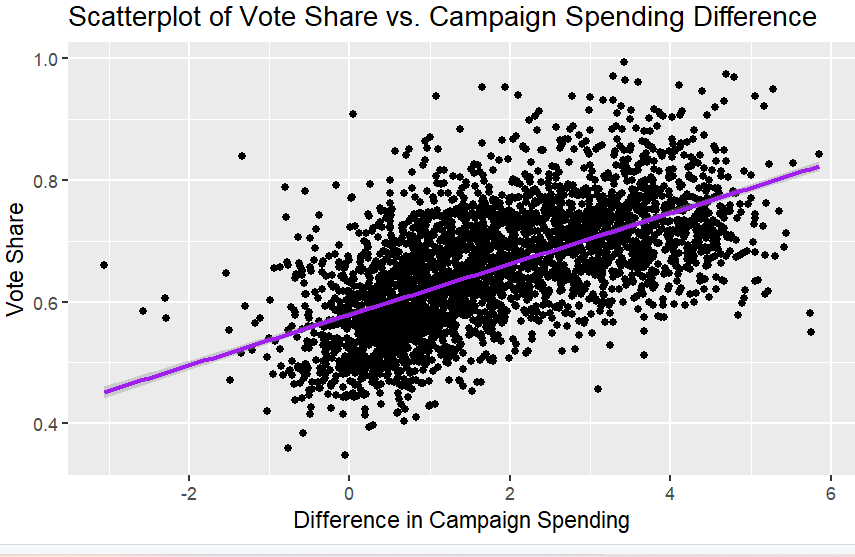
\includegraphics[width=0.8\textwidth]{Question1.png}
	\end{figure}	
		\item Save the residuals of the model in a separate object.		
		\\
			\lstinputlisting[language=R, firstline=48, lastline=49]{PS3_Qin Guo.R}
		\item Write the prediction equation.
			\lstinputlisting[language=R, firstline=51, lastline=56]{PS3_Qin Guo.R}
			\begin{align*}
				voteshare = 0.58 + 0.04 \times \text{difflog}
			\end{align*}
	\end{enumerate}
	

\section*{Question 2}
\noindent We are interested in knowing how the difference between incumbent and challenger's spending and the vote share of the presidential candidate of the incumbent's party are  related.	\vspace{.25cm}
	\begin{enumerate}
		\item Run a regression where the outcome variable is \texttt{presvote} and the explanatory variable is \texttt{difflog}.		\lstinputlisting[language=R, firstline=60, lastline=61]{PS3_Qin Guo.R}
		\item Make a scatterplot of the two variables and add the regression line. 	\lstinputlisting[language=R, firstline=63, lastline=69]{PS3_Qin Guo.R}	
		\begin{figure}[h]
			\centering
			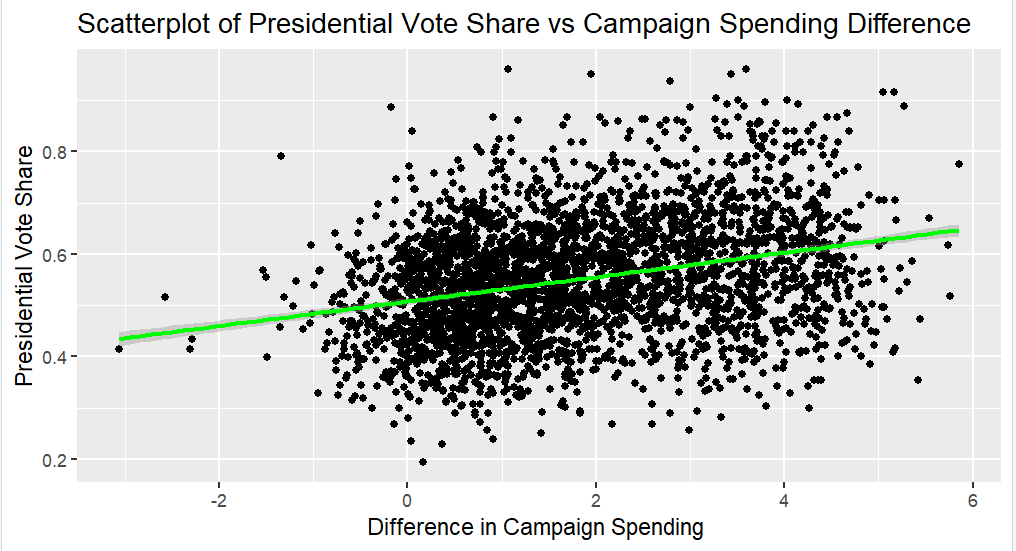
\includegraphics[width=0.8\textwidth]{Question2.png}
     	\end{figure}	
			\vspace{5cm}
		\item Save the residuals of the model in a separate object.	\lstinputlisting[language=R, firstline=71, lastline=72]{PS3_Qin Guo.R}	
		\item Write the prediction equation.
			\lstinputlisting[language=R, firstline=74, lastline=79]{PS3_Qin Guo.R}
				\begin{align*}
				voteshare = 0.51 + 0.02 \times \text{difflog}
			\end{align*}
	\end{enumerate}
	
\section*{Question 3}

\noindent We are interested in knowing how the vote share of the presidential candidate of the incumbent's party is associated with the incumbent's electoral success.
	\vspace{.25cm}
	\begin{enumerate}
		\item Run a regression where the outcome variable is \texttt{voteshare} and the explanatory variable is \texttt{presvote}.	\lstinputlisting[language=R, firstline=83, lastline=84]{PS3_Qin Guo.R}
	
		\item Make a scatterplot of the two variables and add the regression line. 	\lstinputlisting[language=R, firstline=86, lastline=92]{PS3_Qin Guo.R}
		\begin{figure}[h]
			\centering
			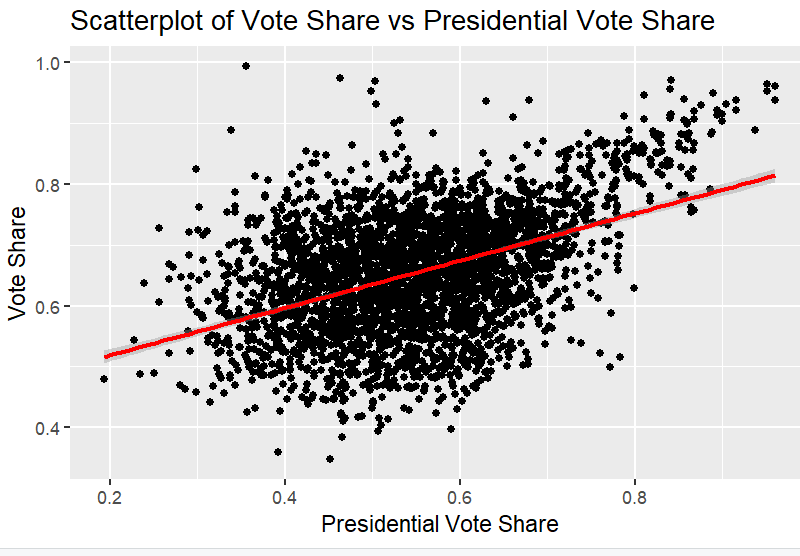
\includegraphics[width=0.8\textwidth]{Question3.png}
		\end{figure}	
			\vspace{3cm}
		\item Write the prediction equation.
			\lstinputlisting[language=R, firstline=94, lastline=99]{PS3_Qin Guo.R}
			\begin{align*}
				voteshare = 0.44 + 0.39 \times \text{presvote}
			\end{align*}
			
	\end{enumerate}
	
\section*{Question 4}
\noindent The residuals from part (a) tell us how much of the variation in \texttt{voteshare} is $not$ explained by the difference in spending between incumbent and challenger. The residuals in part (b) tell us how much of the variation in \texttt{presvote} is $not$ explained by the difference in spending between incumbent and challenger in the district.
	\begin{enumerate}
		\item Run a regression where the outcome variable is the residuals from Question 1 and the explanatory variable is the residuals from Question 2.		\lstinputlisting[language=R, firstline=103, lastline=104]{PS3_Qin Guo.R}
		\item Make a scatterplot of the two residuals and add the regression line. 	\lstinputlisting[language=R, firstline=106, lastline=112]{PS3_Qin Guo.R}
		\begin{figure}[h]
			\centering
			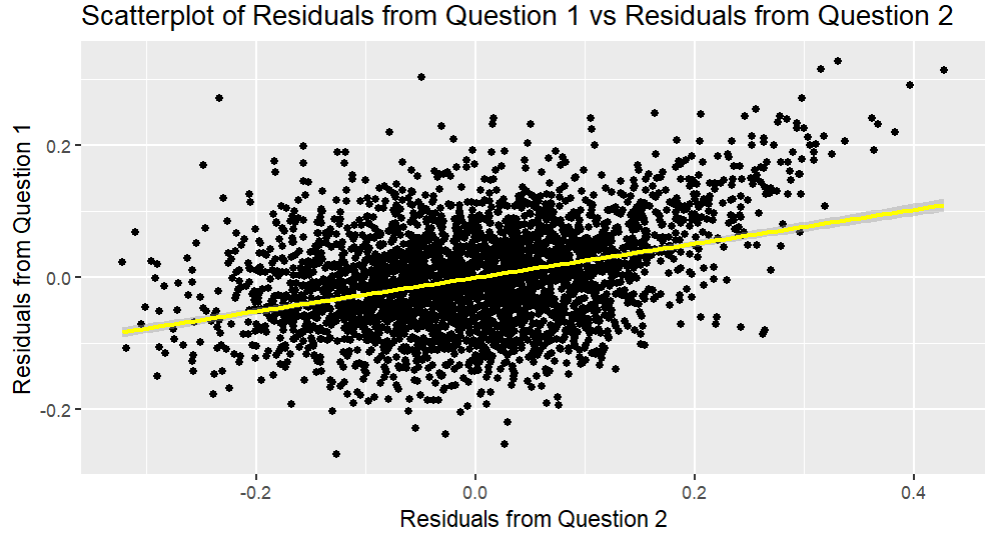
\includegraphics[width=0.8\textwidth]{Question4.png}
		\end{figure}		\vspace{3cm}
		\item Write the prediction equation.
			\lstinputlisting[language=R, firstline=114, lastline=119]{PS3_Qin Guo.R}
			\begin{align*}
				residuals1 = 0 + 0.26 \times \text{residuals2}
			\end{align*}
	\end{enumerate}
	

\section*{Question 5}
\noindent What if the incumbent's vote share is affected by both the president's popularity and the difference in spending between incumbent and challenger? 
	\begin{enumerate}
		\item Run a regression where the outcome variable is the incumbent's \texttt{voteshare} and the explanatory variables are \texttt{difflog} and \texttt{presvote}.	\lstinputlisting[language=R, firstline=123, lastline=124]{PS3_Qin Guo.R}	
		\item Write the prediction equation.	\lstinputlisting[language=R, firstline=126, lastline=132]{PS3_Qin Guo.R}	
		\begin{align*}
			voteshare = 0.45 + 0.04 \times \text{difflog} + 0.26\times \text{presvote}
		\end{align*}
		\item What is it in this output that is identical to the output in Question 4? Why do you think this is the case?
		\vspace{.15cm}
		\noindent
		    \\The identical element in the output of this question  compared to Question 4 is likely the coefficient for presvote.\\
        	Because in this question, we conducted a multiple regression analysis in which we considered both the effects of campaign funding differences (difflog) and the presidential candidate's vote share (presvote) on the incumbent's vote share (voteshare). In this model, we are trying to understand how the presidential candidate's vote share affects the incumbent's vote share after accounting for funding differences. In Question 4, we are actually analyzing the relationship between two residuals: one is the residual of the incumbent's vote share (the part not explained by funding differences in Question 1), and the other is the residual of the presidential candidate's vote share (the part not explained by funding differences in Question 2). This analysis helps us understand the relationship between the presidential candidate's vote share and the incumbent's vote share after excluding the impact of funding differences.\\
        	The key point is that in both cases, we are trying to solve the same mystery: how much impact does the presidential candidate's vote share have on the incumbent's vote share after excluding the impact of funding differences. In question 5, we did this by directly using funding differences and presidential candidate vote share as explanatory variables, whereas in question 4, we did this indirectly by looking at the residuals of the two variables.\\
        	So, despite the different approaches, both analyses are trying to answer the same question, which is why the coefficient of presvote in question 5 is the same as the coefficient of presvote in the residual regression in question 4. This coefficient reflects the net effect of the presidential candidate's vote share on the incumbent's vote share after controlling for funding differences.\\
	\end{enumerate}




\end{document}
